\documentclass[a4paper]{article}

\usepackage[T1]{fontenc}
\usepackage[utf8]{inputenc}
\usepackage[english]{babel}
\usepackage{csquotes}
\usepackage{listings}
\usepackage{multicol}
\lstset{language=c,frame=single,captionpos=b}
\usepackage{hyperref}
\usepackage{amsmath}
\usepackage[backend=biber, sorting=none,maxbibnames=40]{biblatex}
\renewbibmacro{in:}{}
\addbibresource{ref.bib}
\usepackage{graphicx}
\usepackage{placeins}
\usepackage[margin=2.5cm]{geometry}
\usepackage{subcaption}
\usepackage[affil-it]{authblk}

\begin{document}
\title{MPI Assignment: N-body Simulations}
\author{Stefano Sandonà}
\affil{Vrije Universiteit Amsterdam, Holland}
\date{}
		
\maketitle

\section{The N-body problem}
\label{sec:nbody_problem}
Given N celestial objects (bodies) with some properties (mass, initial velocity, radius, ...), the N-body problem consists on the  prediction of the individual motions of these bodies. This is done by measuring the forces that they exert on each other (Coulomb gravity,...). As a result, we obtain a simulation of the behavior of the system over time.  

\section{The sequential algorithm}
\label{sec:seq_algo}
Simplify structure:
\begin{lstlisting}
for each timestep do
	Compute forces between all bodies
	Compute new positions and velocities
\end{lstlisting}

As first thing, we have to discretize the time, so the application knows what to do at certain timestamps. Than for each step, the algorithm computes all the forces between all the bodies. With the resulting forces, the new velocity and positions of all the bodies are updated.

\subsection{Force computation}
\label{sec:force_comp_seq}
This step of the algorithm is the most expensive and determine its complexity.
The forces that bodies exert on each other has to be calculated once per pair of bodies.
\begin{lstlisting}
for (b=0; b<bodyCt; ++b) {
		for (c=b+1; c<bodyCt; ++c) {
			...
\end{lstlisting}
That means with N bodies, we have (N-1)+(N-2)+(N-3)+...+1 pairs, so O(N\textsuperscript{2}) force computations for every timestamp.

\section{Parallel N-body algorithm}
\label{sec:par}
An efficient parallelization of this algorithm is not trivial because for every step we need updated informations from all bodies that are part of our system to calculate the new values. 

\subsection{Bodies distribution}
\label{sec:bodies_distr}
One of the major problems of the parallel algorithms is the load imbalance. If we don't distribute the work fairly between the machines involved in the computation, we'll have some machines idle while others will still work. This problem affects a lot the performance of the application because the overall execution time depends on the last machine that terminate the computation. As each body has to interact with all the others, we have the same amount of work per body, so we just have to find a way to distribute equally the N bodies among all machines. Using a simple \textit{for} construct we can calculate the chunks of bodies to assign to each computational node (number of bodies per node and the boundaries of the chunks).

\begin{lstlisting}
int sum = 0;
for (i = 0; i < numprocs; i++) {
    bodies_per_proc[i] = bodyCt / numprocs;
    if (rem > 0) {
        bodies_per_proc[i]++;
        rem--;
    }
    displs[i] = sum;
    sum += bodies_per_proc[i];
}
\end{lstlisting}

\begin{figure}[ht]
  \centering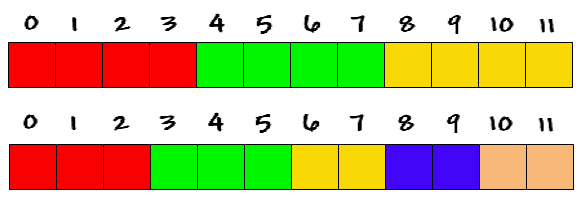
\includegraphics[width=0.6\linewidth]{array_procs_both}
  \caption{12 bodies and 3 computational nodes, 12 bodies and 5 computational nodes}
  \label{fig:3nodes}
\end{figure}
\FloatBarrier

\subsection{The Work repartition}
\label{sec:work_rep}

This is the most critic part of the implementation, from this part depends the efficiency of the algorithm. 
Using a naive approach for every step we could simply using the MPI_Allgatherv operation, to send to all other nodes our updated chunck of bodies and receive all the other chuncks from other nodes.




\begin{figure}[ht]
  \centering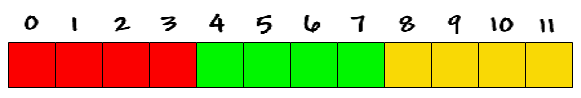
\includegraphics[width=0.6\linewidth]{array_procs_3}
  \caption{12 bodies and 3 computational nodes}
  \label{fig:3nodes}
\end{figure}

\begin{table}[]
\centering
\caption{Node 0}
\label{my-label}
\begin{tabular}{l|llllllll}
block0 & 0-1 & 0-2 & 0-3  & 1-2  & 1-3 & 2-3 &      &      \\ \hline
block1 & 0-4 & 0-5 & 0-6  & 0-7  & 1-4 & 1-5 & 1-6  & 1-7  \\ \hline
block2 & 0-8 & 0-9 & 0-10 & 0-11 & 1-8 & 1-9 & 1-10 & 1-11
\end{tabular}
\end{table}

\begin{table}[]
\centering
\caption{Node 1}
\label{my-label}
\begin{tabular}{l|llllllll}
block0 & 2-4 & 2-5 & 2-6  & 2-7  & 3-4 & 3-5 & 3-6  & 3-7  \\ \hline
block1 & 4-5 & 4-6 & 4-7  & 5-6  & 5-7 & 6-7 &      &      \\ \hline
block2 & 4-8 & 4-9 & 4-10 & 4-11 & 5-8 & 5-9 & 5-10 & 5-11
\end{tabular}
\end{table}

\begin{table}[]
\centering
\caption{Node 2}
\label{my-label}
\begin{tabular}{l|llllllll}
block0 & 2-8 & 2-9  & 2-10 & 2-11 & 3-8  & 3-9   & 3-10 & 3-11 \\ \hline
block1 & 6-8 & 6-9  & 6-10 & 6-11 & 7-8  & 7-9   & 7-10 & 7-11 \\ \hline
block2 & 8-9 & 8-10 & 8-11 & 9-10 & 9-11 & 10-11 &      &     
\end{tabular}
\end{table}

\begin{figure}[ht]
  \centering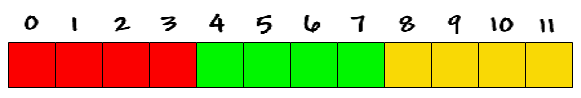
\includegraphics[width=0.6\linewidth]{array_procs_3}
  \caption{12 bodies and 5 computational nodes}
  \label{fig:5nodes}
\end{figure}

\begin{table}[]
\centering
\caption{Node 0}
\label{my-label}
\begin{tabular}{l|llllll}
block0 & 0-1  & 0-2  & 1-2 &  &  &  \\ \hline
block1 & 0-3  & 0-4  & 0-5 &  &  &  \\ \hline
block2 & 0-6  & 0-7  &     &  &  &  \\ \hline
block3 & 0-8  & 0-9  &     &  &  &  \\ \hline
block4 & 0-10 & 0-11 &     &  &  &  
\end{tabular}
\end{table}

\begin{table}[]
\centering
\caption{Node 1}
\label{my-label}
\begin{tabular}{l|llllll}
block0 & 1-3  & 1-4  & 1-5 & 2-3 & 2-4 & 2-5  \\ \hline
block1 & 3-4  & 3-5  & 4-5 &     &     &      \\ \hline
block2 & 3-6  & 3-7  &     &     &     &      \\ \hline
block3 & 3-8  & 3-9  &     &     &     &      \\ \hline
block4 & 3-10 & 3-11 &     &     &     &      
\end{tabular}
\end{table}

\begin{table}[]
\centering
\caption{Node 2}
\label{my-label}
\begin{tabular}{l|llllll}
block0 & 1-6  & 1-7  & 2-6 & 2-7 &  &  \\ \hline
block1 & 4-6  & 4-7  & 5-6 & 5-7 &  &  \\ \hline
block2 & 6-7  &      &     &     &  &  \\ \hline
block3 & 6-8  & 6-9  &     &     &  &  \\ \hline
block4 & 6-10 & 6-11 &     &     &  & 
\end{tabular}
\end{table}

\begin{table}[]
\centering
\caption{My caption}
\label{my-label}
\begin{tabular}{l|llllll}
block0 & 1-8  & 1-9  & 2-8 & 2-9 &  &  \\ \hline
block1 & 4-8  & 4-9  & 5-8 & 5-9 &  &  \\ \hline
block2 & 7-8  & 7-9  &     &     &  &  \\ \hline
block3 & 8-9  &      &     &     &  &  \\ \hline
block4 & 8-10 & 8-11 &     &     &  & 
\end{tabular}
\end{table}

\begin{table}[]
\centering
\caption{Node 3}
\label{my-label}
\begin{tabular}{l|llllll}
block0 & 1-10  & 1-11 & 2-10 & 2-11 &  &  \\ \hline
block1 & 4-10  & 4-11 & 5-10 & 5-11 &  &  \\ \hline
block2 & 7-10  & 7-11 &      &      &  &  \\ \hline
block3 & 9-10  & 9-11 &      &      &  &  \\ \hline
block4 & 10-11 &      &      &      &  & 
\end{tabular}
\end{table}

\printbibliography 

\end{document}